We have seen since the first chapter of these notes that \textbf{Cyber-physical systems} are sets of interconnected devices which
take measurements from the physical world through the use of sensors. Such framework is \textbf{intrinsically distributed} even in the measurement stage that in the processing stages.
\section{Toward the Fusion Center removal}


\noindent
In the first part of this course we have seen that there was a 
\textbf{fusion center} which collects and processes all the data (it can be for example a computer connected via Wi-Fi), another way to perform processing in the CPSs framework is the \textbf{distributed way}, then by using \textbf{distributed} (or \textbf{decentralized) algorithms}. The figure below shows the differences between a centralized and a distributed setting, respectively:

\begin{figure}[h]
    \centering
    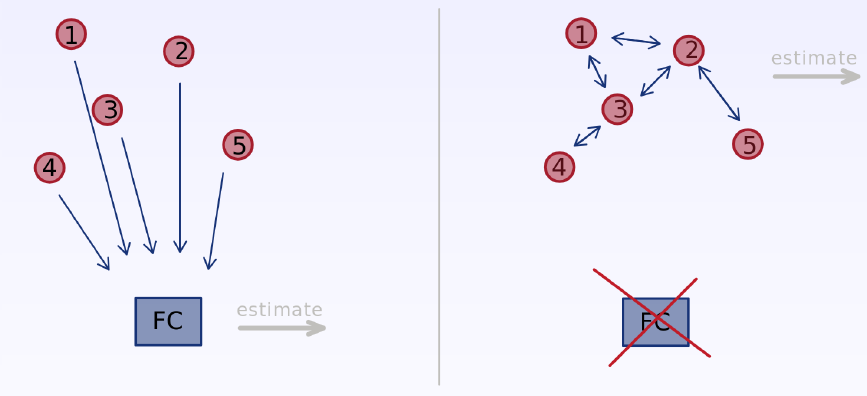
\includegraphics[scale=0.6]{images/Dist_Centr.png}
    \caption{Centralized and Distributed processing}
\end{figure}
\begin{itemize}
    \item In the first case all the data are conveyed to the fusion center to which is assigned the work of collecting and processing it; by using centralized algorithms some estimates can be given;
    \item In the second case of a \textbf{distributed} approach, the agents (or nodes)  cooperate by \textbf{exchanging information} in order to perform the elaboration.
\end{itemize}
In this last chapter of the 'Modeling' part, we are going toward the \textbf{removal of the Fusion Center} in order to understand the methods can be used for \textit{decentralized processing}.

\subsection{Motivations} 
The motivation that guide us to the decentralization, is quite practical: a large number of \textbf{cheap} interconnected devices which cooperate is better than few \textbf{expensive} devices. The adjectives \textbf{cheap/expensive} have to be declined in term of: computational capability, accuracy, power consumption and so on. Decentralized systems are: (i) \textbf{more robust} to failures, (ii) cheaper to maintain. However some \textbf{distributed algorithms} are needed.
In the figure below are presented further information about advantages and disadvantages between the two approaches.\\

\begin{figure}[h]
    \centering
    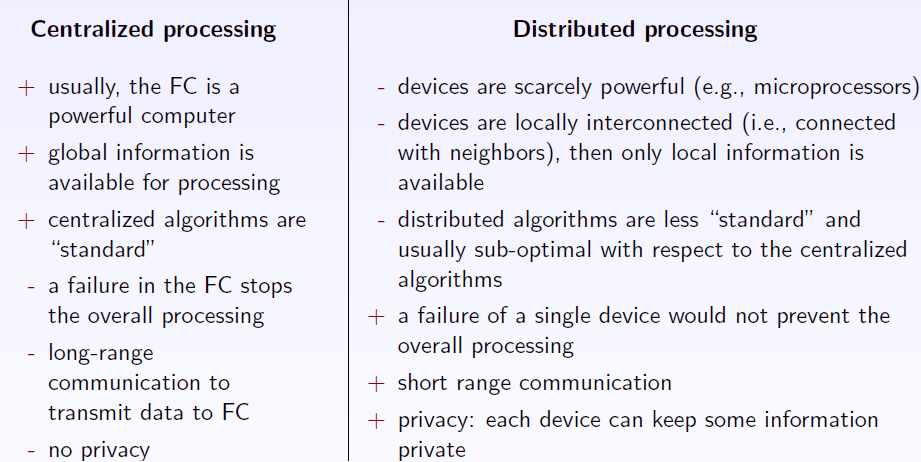
\includegraphics[scale=0.8]{images/Pros_Cons.png}
    \caption{Pros and cons}
\end{figure}


It is quite common that in this field one talk about \textbf{multi-agent systems}. They are in a nutshell collections of devices that communicate to \textbf{achieve a common goal} (we will see that this concept is strongly connected to the  \textbf{consensus}). An \textbf{agent/node} is a device with other agents and takes autonomous decisions. 

\section{Distributed Least Squares (I)}
As we understood is the problem of estimate the state $\tilde{x}\in \mathbb{R}^n$ given linear measurements of the type $y=C\tilde{x}+\eta$, where $\eta$ is a generic noise of measurement. We can use a Least-Square approach:
\begin{equation}
    \min_{x \in \mathbb{R}^n} \Vert y-Cx \Vert_2^2
\end{equation}
The minimizer $x^*$ gives us the estimate of $\tilde{x}$. We have removed the Fusion Center(FC) we cannot run any algorithm (eg. Gradient Descent) to compute the estimate. In the scenario in which the agents are \textbf{sensors}, for example each sensor has its own $C_i$ (the $i-th$ row of the matrix C) and its own (distributed) measurement. It is remarkable that such quantities are not shared due to issues related to \textbf{privacy} and \textbf{storage capacity}! However another 'smaller' information can be exploited: the local estimate $x^{(i)} \in \mathbb{R}^n$ of the state. On the other hand if each sensor node $i$ solved the LS problem, the resulting estimated would have been very inaccurate. \textbf{Solution} $\Leftarrow$ we need \textbf{cooperation} among sensor nodes.

\subsection*{Math tool: Graphs}
At this point, our next aim is to find a \textbf{model} to analyze the cooperation among agents. The best way is using a very powerful tool from the discrete Maths: Graphs. Essential definitions and features are given in this paragraph in order to continue the discussion. 
\begin{figure}[h]
    \centering
    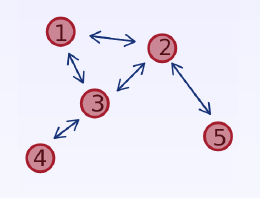
\includegraphics[scale=1.2]{images/Graph.png}
    \caption{Example of a graph}    
\end{figure}

\noindent
A \textbf{directed graph} $\mathcal{G}=(\mathcal{N}, \mathcal{E})$ is given by a couple of sets:
\begin{itemize}
    \item A set of \textbf{nodes or vertices} $\mathcal{N}=\{1,2,..., q\}$
    \item A set of \textbf{links or edges} $\mathcal{E}\subseteq\mathcal{N} \times  \mathcal{N}.$
\end{itemize}
If $(i,j)\in\mathcal{E}$ we say that $(i,j)$ are neighbours. We define the \textbf{neighbourhood} of a nodes as the set of the nodes from which it receives information, the vertices from which derive the \textbf{incoming edges}. Just to give an example, the neighbourhood of 3 is the set $\mathcal{N}_3=\{1,2,4\}$. \\
Our aims bring us to make a consideration if there is an edge between two nodes, this means that they communicate.\\
Some other feature are relevant for our purposes: 
\begin{itemize}
    \item A graph is said to be \textbf{complete} if $\mathcal{E}=\mathcal{E} \times \mathcal{E}$; 
    \item The graphs we will analyze are assumed to be \textbf{strongly connected} that is there is always a path between each pair of nodes; 
\end{itemize}

\subsection{Introduction to Distributed Gradient Descent}
For the aim of decentralizing the agents share their \textbf{local estimate} $x^{(i)}(k)$ which denotes the {\color{red} estimate of $\tilde{x}$ at time $k$}, let us assume for simplicity and without loss of generality, that such estimate is a \textbf{scalar}. \\
Once a generic sensor receives the estimate coming from its neighbourhood $\mathcal{N}_i$, it computes a \textbf{local mean}
\begin{equation}
    \bar{x}^{(i)}(k) = \frac{1}{\vert \mathcal{N}_i \vert} \sum_{j\in\mathcal{N}_i} x^{(j)}(k)
\end{equation}
where $\vert \mathcal{N}_i \vert$ is the cardinality of the neighbourhood. Despite it is true that a local solution of the LS problem (by using the Gradient Descent) would give an inaccurate estimate, the partial functional $F_i=y_i-C_ix$ can be used to run a step of the gradient descent to update the estimate by using the information of the calculated local mean. More precisely each node executes
\begin{equation}    \label{eq:DGD_1}
    x^{(i)}(k+1) = \bar{x}^{(i)}(k) -\tau \nabla (x^{i}(k))
\end{equation}

This equation raises the problem known as the \textbf{Distributed Gradient Descent} which mixes: (i) \textbf{local} communication by performing the local mean, (ii) individual processing for the gradient step. By iterating this computation an estimate of the global state can be achieved. \\
{\color{blue}Note that: we assume that in the neighbourhood of a vertex there is the vertex itself, as if there was a self-loop}.
One can wonder: {\color{red} Why local mean and not another metric?} This observation gives the motivation to entry in more details talking about \textbf{Consensus algorithm}.

\section{The Consensus algorithm}
\noindent
The central point is: what should it happen if I iterate the local mean? Under some conditions for each node $i=1,...,q$
for a certain time $k\rightarrow\infty$
\begin{align*}
    &x^{(1)}(k) \rightarrow x^*\\
    &x^{(2)}(k) \rightarrow x^*\\
    &\vdots\\ \vdots
    &x^{(q)}(k) \rightarrow x^*
\end{align*}
Then, the nodes estimate the same global quantity $x^*$, they reach a \textbf{consensus}. In some cases we are interested in   \textbf{average consensus}, that is
\begin{equation}
    x^*=\frac{1}{q}\sum_{i=1}^q x^{(i)}(0)
\end{equation}
Let us consider an example for a graph of only three agents which is showed in the figure below (it has been used the \texttt{digraph} command of Matlab):
\begin{figure}[h]
    \centering
    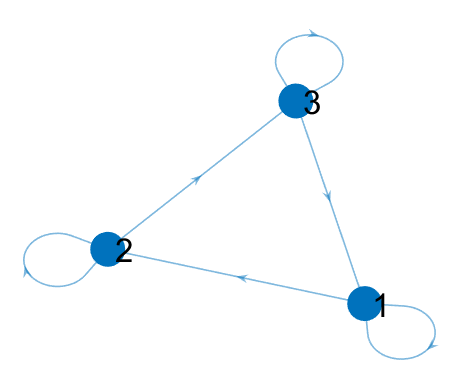
\includegraphics[scale=0.7]{images/Es_graph.png}
\end{figure}

At a certain time $k$ we have the following local means:
\begin{equation}    \label{eq: local_means}
    \begin{aligned}
        &x^{(1)}(k+1)=\bar{x}^{(1)} = \frac{1}{2} (x^{(1)}(k)+x^{(3)}(k))\\
        &x^{(2)}(k+1)=\bar{x}^{(2)} = \frac{1}{2} (x^{(1)}(k)+x^{(2)}(k))\\
        &x^{(3)}(k+1)=\bar{x}^{(2)} = \frac{1}{2} (x^{(3)}(k)+x^{(2)}(k))
    \end{aligned}
\end{equation}

\noindent
We have for each node a \textbf{local weighted mean} (only the neighbours), each weight can be represented by a scalar $Q_{ij}$ and at this point the system above becomes
\begin{equation}
    \begin{aligned}
        &x^{(1)}(k+1)= Q_{11} x^{(1)}(k)+Q_{13}x^{(3)}(k)\\
        &x^{(2)}(k+1)= Q_{11} x^{(1)}(k)+Q_{12}x^{(2)}(k)\\
        &x^{(3)}(k+1)= Q_{12} x^{(2)}(k)+Q_{13}x^{(3)}(k)\\
    \end{aligned}
\end{equation}
By collecting the $Q_{ij}$ in a matrix 
$$Q=\begin{pmatrix}
    Q_{11}&Q_{12}&Q_{13}\\
    Q_{21}&Q_{22}&Q_{23}\\
    Q_{31}&Q_{32}&Q_{33}
\end{pmatrix}
    \in\mathbb{R}^{3,3}$$
we can represent the system (\ref{eq: local_means}) in a matrix form as
\begin{equation}
    x(k+1)=Qx(k)
\end{equation}
which summarize in a succinct way the Consensus algorithm where
$$x(k)=\begin{pmatrix} x^{(1)}(k)\\x^{(2)}(k)\\\vdots\\x^{(q)}(k) \end{pmatrix}$$ 

An important observation can be done on the matrix $Q$, each element $Q_{ij}\le 0$, if $Q_{ij}=0$ then there is no link between $i$ and $j$. Moreover for each row the sum of the element is equal to one, that is $\sum_{j=1}^q x_{ij}=1$ (convex combination), such a matrix is called \textbf{stochastic matrix} (or row stochastic). We can observe that the Consensus problem is an LTI DT dynamical system and its formulation is completely coincident with the formulation of \textbf{Page Rank algorithm} and \textbf{Markov Chains}. Now we are going to investigate the fact that the properties of the matrix $Q$ are very important.

\subsection{Properties of stochastic matrices}
The following properties are relevant for our purposes:
\begin{itemize}
\item Let Spec($Q$)=$\{\lambda_1, ..., \lambda_q\}$ be the set of the eigenvalues of the stochastic matrix $Q$, it holds that $\lambda_i \le 1, \ i=1,...,q$, so the \textit{spectral radius} of Q is $\rho(Q)=\max_{i=1,...,q}\{\vert\lambda_i \vert\}=1$
\item Let $\mathbf{1}=(1,1,...,1)^T$, $Q\mathbf{1}=1$ this is equivalent to state that $\mathbf{1}\in\mathbb{R}^{q}$ is an eigenvector of $Q$ and its associated eigenvalues is $\lambda=1$, this results in a non-asymptotical stability of the dynamical system associated to the consensus problem;
\item The first eigenvalue of $Q$ is denoted with $\lambda_{PF}$ and it is called \textbf{Perron-Frobenius} or \textbf{leading eigenvalue}.
\end{itemize}

\noindent
Starting from  $k=0$ Let us have a look to the evolution of the system, what is its behaviour for $k\to\infty$? 
\begin{align*}
    &x(0)\\
    &x(1)=Qx(0)\\
    &x(2)=Qx(1)=Q^2x(0)\\
    &\dots\\
    &x(k+1)=Q^{k+1} x(0)
\end{align*}
We can note that  it depends only on the power of the matrix $Q$. Some examples can be useful to try explaining this behaviour.\\

\noindent
{\color{red}\textbf{Example 1}}
\begin{align*}
    Q=\begin{pmatrix}
        0.1&0.2&0.7\\1&0&0\\0.3&0.3&0.4
    \end{pmatrix} \Longrightarrow 
    \lim_{k\to\infty} Q^k=\begin{pmatrix}
        0.3681&0.2025&0.4294\\
        0.3681&0.2025&0.4294\\
        0.3681&0.2025&0.4294
    \end{pmatrix}
\end{align*}
The limit has been computed by using numerical techniques, now we know what is the behaviour for $k\to\infty$, because
\begin{equation*}
    \lim_{k\to\infty} x(k)=\lim_{k\to\infty} Q^kx(0) = [0.3681x^{(1)}(0)+0.2025x^{(2)}(0)+0.4294x^{(3)}(0)] \mathbf{1}
\end{equation*}
In this way we reach the consensus, in the sense that the value of the local mean converge to a single value.\\

\noindent
{\color{red}\textbf{Example 2}}
\begin{align*}
    Q=\begin{pmatrix}
        0.1&0.2&0.7\\1&0&0\\0&0&1
    \end{pmatrix} \Longrightarrow 
    \lim_{k\to\infty} Q^k=\begin{pmatrix}
        0&0&1\\
        0&0&1\\
        0&0&1
    \end{pmatrix}
\end{align*}
Even in this case we analyze the behaviour for increasing $k$ and we can note that:
$$
    \lim_{k\to\infty} x(k)=\lim_{k\to\infty} Q^kx(0)=x^{(3)}(0) \mathbf{1}
$$
Since the matrix $Q$ has got three identic rows, it achieves the consensus.\\

\noindent
{\color{red}\textbf{Example 3}}
\begin{align*}
    Q=\begin{pmatrix}
        1&0&0\\
        1&0&0\\
        0&0&1
    \end{pmatrix}  \Longrightarrow
    \lim_{k\to\infty} Q^k = \begin{pmatrix}
        1&0&0\\
        1&0&0\\
        0&0&1
    \end{pmatrix}
\end{align*}
In this case nothing change, as $k$ increases, the global decision is not achieved. In particular: $$\lim_{k\to\infty} x(k)=\begin{pmatrix}
    x^{(1)}(0)\\
    x^{(2)}(0)\\
    x^{(3)}(0)
\end{pmatrix}$$

\noindent
{\color{red}\textbf{Example 4}}\\
\begin{equation*}
    Q=\begin{pmatrix}
        0.1&0.2&0.7\\
        0.2&0.8&0\\
        0.7&0&0.3
    \end{pmatrix} \Longrightarrow 
    \lim_{k\to\infty}Q^{k}x(0)=\frac{1}{3} \bigg[\ 
    \sum_{i=1}^3 x^{(i)}(0) 
    \bigg] \mathbf{1}
\end{equation*}
This is the case in which we have the \textbf{average consensus}, this is due to the fact the matrix $Q$ is \textbf{doubly stochastic} because is both stochastic and symmetric, this reveal a property about the structure of the graph: it is undirected. \\

After these examples have been given, we are ready to give the following definitions:\\

%Per disegnare il box
\hspace*{-5mm}
\begin{tikzpicture}
\node [mybox] (box){%
    \begin{minipage}{.96\textwidth}     %Larghezza del box
        {
            \large{
                {\color{red}\underline{\textbf{Definition (CONSENSUS)}}}\\
            Given the dynamical system $x(k+1)=Qx(k)$, with $Q\in\mathbb{R}^{q,q}$, $x(k)\in\mathbb{R}^n$, we say that $Q$ achieve the consensus if there exists an $\alpha\in\mathbb{R}$ such that
            $$\lim_{k\to\infty} x(k)=\alpha\mathbf{1}$$
            Instead we reach the \textbf{average consensus} if $$\alpha=\frac{1}{q} \sum_{i=1}^q x^{(i)}(0)$$
            }
        }
            
    \end{minipage}
};
\end{tikzpicture}%

\noindent
The stochastic matrix $Q$ is so important that we can have sufficient conditions for consensus only by analyzing its eigenvalues. In particular the following theorem it has been demonstrated:\\

\hspace*{-5mm}
\begin{tikzpicture}
\node [mybox] (box){%
    \begin{minipage}{.96\textwidth}     %Larghezza del box
        { \large{
            \textbf{Theorem (Perron-Frobenius)}\\
            Let $\lambda_1=\lambda_{PF}=1 \ \text{and} \ \lambda_1>\vert \lambda_2 \vert \le ... \le \vert \lambda_q \vert$, then $Q$ achieves \textbf{consensus}.
        }}
    \end{minipage}
};
\end{tikzpicture}%

\noindent
\textbf{Proof (for diagonalizable Q)}
\textit{
    Let us assume for simplicity that Q is diagonalizable in a way that is simpler doing the computation $Q^k$. If $Q$ is diagonalizable, it is similar to a diagonal matrix that is
    \begin{align*}
        &Q=V \Lambda V^{-1}
         = V \begin{pmatrix}
            1&0&...&0\\
            0&\lambda_2&...&0\\
            &\vdots&\vdots&\ddots\\
            0&0&...&\lambda_q
         \end{pmatrix} V^{-1}\\
         &Q^{k}=V \Lambda^k V^-1 = V \begin{pmatrix}
            1&0&...&0\\
            0&\lambda_2^q&...&0\\
            &\vdots&\vdots&\ddots\\
            0&0&...&\lambda_q^q
        \end{pmatrix} V^{-1} \to
        V \begin{pmatrix}
            1&0&...&0\\
            0&0&...&0\\
            &\vdots&\vdots&\ddots\\
            0&0&...&0
        \end{pmatrix} V^{-1}=\\
        &=\begin{pmatrix}
            V_{11}&0&...&0\\
            V_{21}&0&...&0\\
            &\vdots&\vdots&\ddots\\
            V_{n1}&0&...&0
        \end{pmatrix} V^{-1}=\frac{1}{\sqrt{q}}\begin{pmatrix}
            1&0&...&0\\
            1&0&...&0\\
            &\vdots&\vdots&\ddots\\
            1&0&...&0
        \end{pmatrix} V^{-1}=\begin{pmatrix}
            \beta_1&\beta_2&...&\beta_q\\
            \beta_1&\beta_2&...&\beta_q\\
            \vdots& & \vdots\\
            \beta_1&\beta_2&...&\beta_q\\
        \end{pmatrix}
    \end{align*} 
    At this point given $Q^k$, we can compute the limit
    \begin{equation*}
        \lim_{k\to\infty} Q^kx(0)=\sum_{j=1}^q \beta_j x^{(j)}(0) \mathbf{1} \Longrightarrow \text{\textbf{we reach consensus}}
    \end{equation*}
} 

\noindent
In a similar way we can give a sufficient condition for achieving the \textbf{average consensus}: \\

\hspace*{-5mm}
\begin{tikzpicture}
\node [mybox] (box){%
    \begin{minipage}{.96\textwidth}     %Larghezza del box
        \textbf{Theorem}\\
        Let Q be a doubly stochastic matrix. Let $\lambda_1=\lambda_{PF}=1 \ \text{and} \ \lambda_1>\vert \lambda_2 \vert \le ... \le \vert \lambda_q \vert$. Then $Q$ achieves \textbf{average consensus}.
    \end{minipage}
};
\end{tikzpicture}%

\noindent
\textbf{Proof}\\
\textit{
    In general for a symmetric matrix 
    \begin{align*}
        &Q=V \Lambda V^{T}
         = V \begin{pmatrix}
            1&0&...&0\\
            0&\lambda_2&...&0\\
            &\vdots&\vdots&\ddots\\
            0&0&...&\lambda_q
         \end{pmatrix} V^{-1}\\
         &Q^{k}=V \Lambda^k V^-1 = V \begin{pmatrix}
            1&0&...&0\\
            0&\lambda_2^q&...&0\\
            &\vdots&\vdots&\ddots\\
            0&0&...&\lambda_q^q
        \end{pmatrix} V^{T} \to
        V \begin{pmatrix}
            1&0&...&0\\
            0&0&...&0\\
            &\vdots&\vdots&\ddots\\
            0&0&...&0
        \end{pmatrix} V^{T}=\\
        &=\begin{pmatrix}
            V_{11}&0&...&0\\
            V_{21}&0&...&0\\
            &\vdots&\vdots&\ddots\\
            V_{n1}&0&...&0
        \end{pmatrix} V^{T}=\frac{1}{\sqrt{q}}\begin{pmatrix}
            1&0&...&0\\
            1&0&...&0\\
            &\vdots&\vdots&\ddots\\
            1&0&...&0
        \end{pmatrix} V^{T}=\frac{1}{q}
        \begin{pmatrix}
            1&1&...&1\\
            1&1&...&1\\
            \vdots& & \vdots\\
            1&1&...&1\\
        \end{pmatrix}
    \end{align*} 
    At this point given $Q^k$, we can compute the limit
    \begin{equation*}
        \lim_{k\to\infty} Q^kx(0)=\frac{1}{q}\sum_{j=1}^q x^{(j)}(0) \mathbf{1} \Longrightarrow \text{\textbf{we reach average consensus}}
    \end{equation*}
}

\subsection{On the connectivity}
What is the relationship between consensus and the graph topology? In order to investigate such aspects, let us take some of the matrices $Q$ of the previous examples.

{\color{blue}\subsubsection{Strongly connected graphs}}
Let us consider the following $Q$ matrix:
\begin{equation*}
    Q=\begin{pmatrix}
        0.1&0.2&0.7\\1&0&0\\0.3&0.3&0.4
    \end{pmatrix}
\end{equation*}
The associated graph is the following: 
\begin{figure}[h]
    \centering
    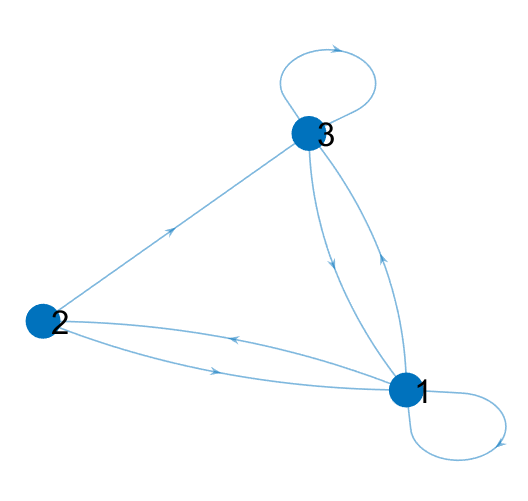
\includegraphics[scale=0.6]{images/Es1_gr.png}
\end{figure}
\noindent
We can note that it is \textbf{strongly connected}, we can give as a result that 
\textbf{each stochastic matrix related to a strongly connected graph reaches consensus}, for the properties which are required from the Perron-Frobenius theorem.

{\color{blue}\subsubsection{Leader-follower}}
From the \textbf{Example 2} we had the following matrix:
\begin{equation*}
    Q=\begin{pmatrix}
        0.1&0.2&0.7\\1&0&0\\0&0&1
    \end{pmatrix}
\end{equation*}
From the limit we can note that the node 3 does not change its own state and the consensus is a global mean which depends only on its state, for this reason can be recognized as a \textbf{leader agent} that propagates its own information without receiving nothing. The other agents are the \textbf{follower nodes}. The associated graph shows the exposed property:
\begin{figure}[h]
    \centering
    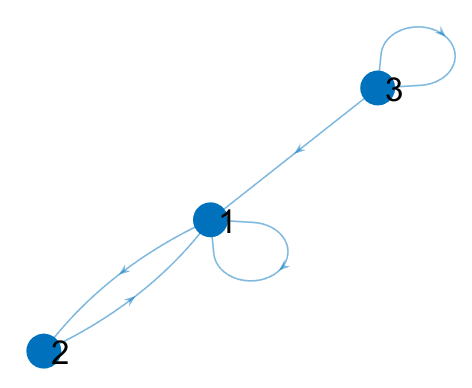
\includegraphics[scale=0.7]{images/Leader_follower.png}
\end{figure}

{\color{blue}\subsubsection{The importance of $Q_{ij}$ magnitude}}
Experimental results are showing that the specific magnitude of  $Q_{ij}$ plays not a fundamental role for the fact that a system may reach the consensus. However, in some situations might be important taking into account even the weight of a certain edge. Let us suppose that on a link there is an attack in the sense that one of the sensors spread the value of the state corrupted by an attack $a$, in those situations, the reduction in magnitude of $Q_{ij}$ can be crucial for the secure estimation of the  state.

\subsection{Convergence rate of the Consensus algorithm}
In order to conclude the explanation obout \textit{Consensus}, we give another important result that help us to estimate the convergence of the Consensus Algorithm.\\

\hspace*{-5mm}
\begin{tikzpicture}
\node [mybox] (box){%
    \begin{minipage}{.96\textwidth}     %Larghezza del box
            {\large{
                \textbf{Theorem (convergence rate of Consensus)}\\

                The convergence rate of the \textit{consensus algorithm} is determined by the \textbf{essential spectral radius} \texttt{esr}($Q$) which is the second \textbf{largest eigenvalue in magnitude}.
            }}
    \end{minipage}
};
\end{tikzpicture}%


\section{Uses of the Consensus algorithm}

\subsection{Distributed Least-Squares (II) and Distributed Gradient Descent}
The attempt which this paragraph try to meet is that of understand and formalize the problem of the \textbf{distributed least squares} just mentioned at the beginning, using also the notions introduced talking about Consensus algorithm.\\
At first, in order to generalize the problem, let us consider the following \textit{convex optimization problem}
\begin{equation}
    \min_{x\in\mathbb{R}^n} F(x)
\end{equation}
where $F:\mathbb{R}^n\to\mathbb{R}$ is a \textbf{convex function}. If $F(x)$ is a the sum of several convex functions, it is called a \textbf{composite functional}
\begin{equation}
    F(x)=\sum_{i=1}^q {F_i(x)}
\end{equation}
In our case our functional $F(x)$ is the Least-Square functional which can be separated into different convex functionals, in the following way
\begin{align}
    F(x)=\Vert Cx-y \Vert_2^2=\sum_{i=1}^q (C_ix-y_i)^2\\
    F_i(x):=(C_ix-y_i)^2
\end{align}

\subsection{Problem $\mathcal{P}$: distributed minimization of composite functionals}
We want to solve the problem
\begin{equation*}
    \min_{x\in\mathbb{R}^n}  \sum_{i=1}^q F_i(x) 
\end{equation*}
under the following assumption: 
\begin{enumerate}
    \item each agent knows its own part of the functional $F_i$
    \item each agent $i$ collaborate and share its own local estimate $x^{(i)}\in\mathbb{R}^n$, while no information on $F_i$ is shared.
    \item The local estimate is updated:
    \begin{enumerate}
        \item Using the functional $F_i$, by computing its \textbf{gradient}
        \item By collecting the information from neighbours.
    \end{enumerate}
\end{enumerate}

If $F(x)$ is convex and differentiable, we can apply the Gradient Descent algorithm in order to reach the \textbf{global minimum} under certain condition. The further step is decentralize the GD as follows:\\

\hspace*{-5mm}
\begin{tikzpicture}
\node [mybox] (box){%
    \begin{minipage}{.96\textwidth}     %Larghezza del box
            {\large{
                {\color{red} \centering\textbf{DISTRIBUTED GRADIENT DESCENT (DGD)}\\}
               

                At each time k, the agent $i$ holds a local estimate $x^{i}(k)\in \mathbb{R}^n$\\
                For $k=1,..., T_{max}$\\
                For each agent $i=1,...,q$, the following steps  are performed:
                \begin{enumerate}
                    \item {\color{red}\textbf{Individual step}}: each agent computes its own gradient 
                    ${u^{(i)}(k)=\nabla F_i(x^{(i)}(k))}$
                    \item {\color{red}\textbf{Consensus step}}
                    a \textbf{weighted local mean} of the neighbours' state is computed 
                    \begin{equation*}
                        \bar{x}^{(i)}(k)=\sum_{j=1}^q {Q_{i,j} x^{(j)}(k)}
                    \end{equation*}
                    \item {\color{red}\textbf{"Merge" step}}: $x^{(i)}(k+1)=\bar{x}^{(i)}(k)- \tau u^{(i)}(k)$
                \end{enumerate}
            }}
    \end{minipage}
};
\end{tikzpicture}%

\noindent
\\The just presented definition was a theoretical one, but \textbf{in practice} between the first and the second step, there is a 2-phase \textbf{Communication step} in which each agent: {\color{red}(i)} broadcasts its own local estimate to the neighbourhood $\mathcal{N}_i$; {\color{red}(ii)} receives from the other agents the local estimate. Once this phase is concluded the \textbf{Consensus step} can be done. In real world applications, some communication delays ought to be taken into account, but for our purposes we are allowed to neglect them.

{\color{blue}
\subsubsection*{On the convergence of DGD}
}

The analysis of the convergence of \textbf{Distributed Gradient Descent} is quite challenging. In some papers the study on the convergence is done focusing the attention on the \textbf{stopped model}, that is, after a certain time $T_s$ the agents stop the computation of the gradient $\longrightarrow$ for $k>T_s$, the DGD consensus become a consensus algorithm. \\
If $x^*= \text{arg}\min_{x\in\mathbb{R}^n} \sum_{i=1}^q F_i(x)$ is the optimal solution and $z^*$ is the solution obtaindd by DGD, then for certain constant $c$ we can have the \textbf{convergence} in the sense that
\begin{equation*}
    \bigg\vert \sum_{i=1}^q F_i(x^*) - \sum_{i=1}^q F_i(z^*)\bigg\vert < c
\end{equation*}

\subsection{Distributed ISTA (DISTA)}
{\color{cyan}
\textbf{What if we had the LASSO functional instead of the Least-Squares one?}
}
\\
We are talking about the well-known least-squares functional to which an $\ell_1$-regularization is added. This results in the fact that the Distributed gradient descent is unusable the $\ell_1$-norm is not differentiable! 

We can adapt the ISTA algorithm in a distributed context by doing some trivial modifications, the operator $\mathbb{S}_{\lambda\tau}$ (shrinkage and thresholding) has to be used. Recalling that we want to minimize the functional 
\begin{equation*}
    F(x)=\Vert y-Ax \Vert_2^2 + \lambda \Vert x \Vert_1
\end{equation*}
now is provided the algorithm to recover in a distributed way a sparse solution. 


\hspace*{-5mm}
\begin{tikzpicture}
\node [mybox] (box){%
    \begin{minipage}{.96\textwidth}     %Larghezza del box
        {\large{
            {\color{red}  \centering\textbf{ 
                 Distributed Iterative Soft Thresholding algorithm (DISTA)}
            }
            \begin{enumerate}
                \item {\color{red} \textbf{Initialization}}: $x^{(i)}(0)\in \mathbb{R}^n$ (eg. $x^{(i)}(0)=0$) 
                \item For $k=1,..., T_{max}$
                \item For each agent $i=1,...,q$
                {\color{blue}
                \begin{equation*}
                    x^{(i)}(k+1) = \mathbb{S}_{\lambda\tau} 
                    \bigg[ 
                        \sum_{i=1}^q Q_{i,j}x^{(j)}(k) +
                        \tau A_i^T(y_i-A_ix^{(i)}(k))
                    \bigg]
                \end{equation*}
                }
                
            \end{enumerate}
        }}
    \end{minipage}
};
\end{tikzpicture}%

{\color{red}
\subsubsection*{DISTA and Secure State Estimation of CPSs}
}

\noindent
By doing the proper adjustments to the LASSO functional, we can use the DISTA algorithm for \textbf{RSS-fingerprinting localization} and in general for the problem of \textbf{Distributed Secure State Estimation of CPSs under attacks}. [It is important to note that that we are now in the \textbf{static setting} and so we assume that no observers are employed, the integration between decentralization and dynamic approach passing through the use of a \textit{sparse observer} is different and challenging!]  

